\begin{figure}[h]
    \centering
    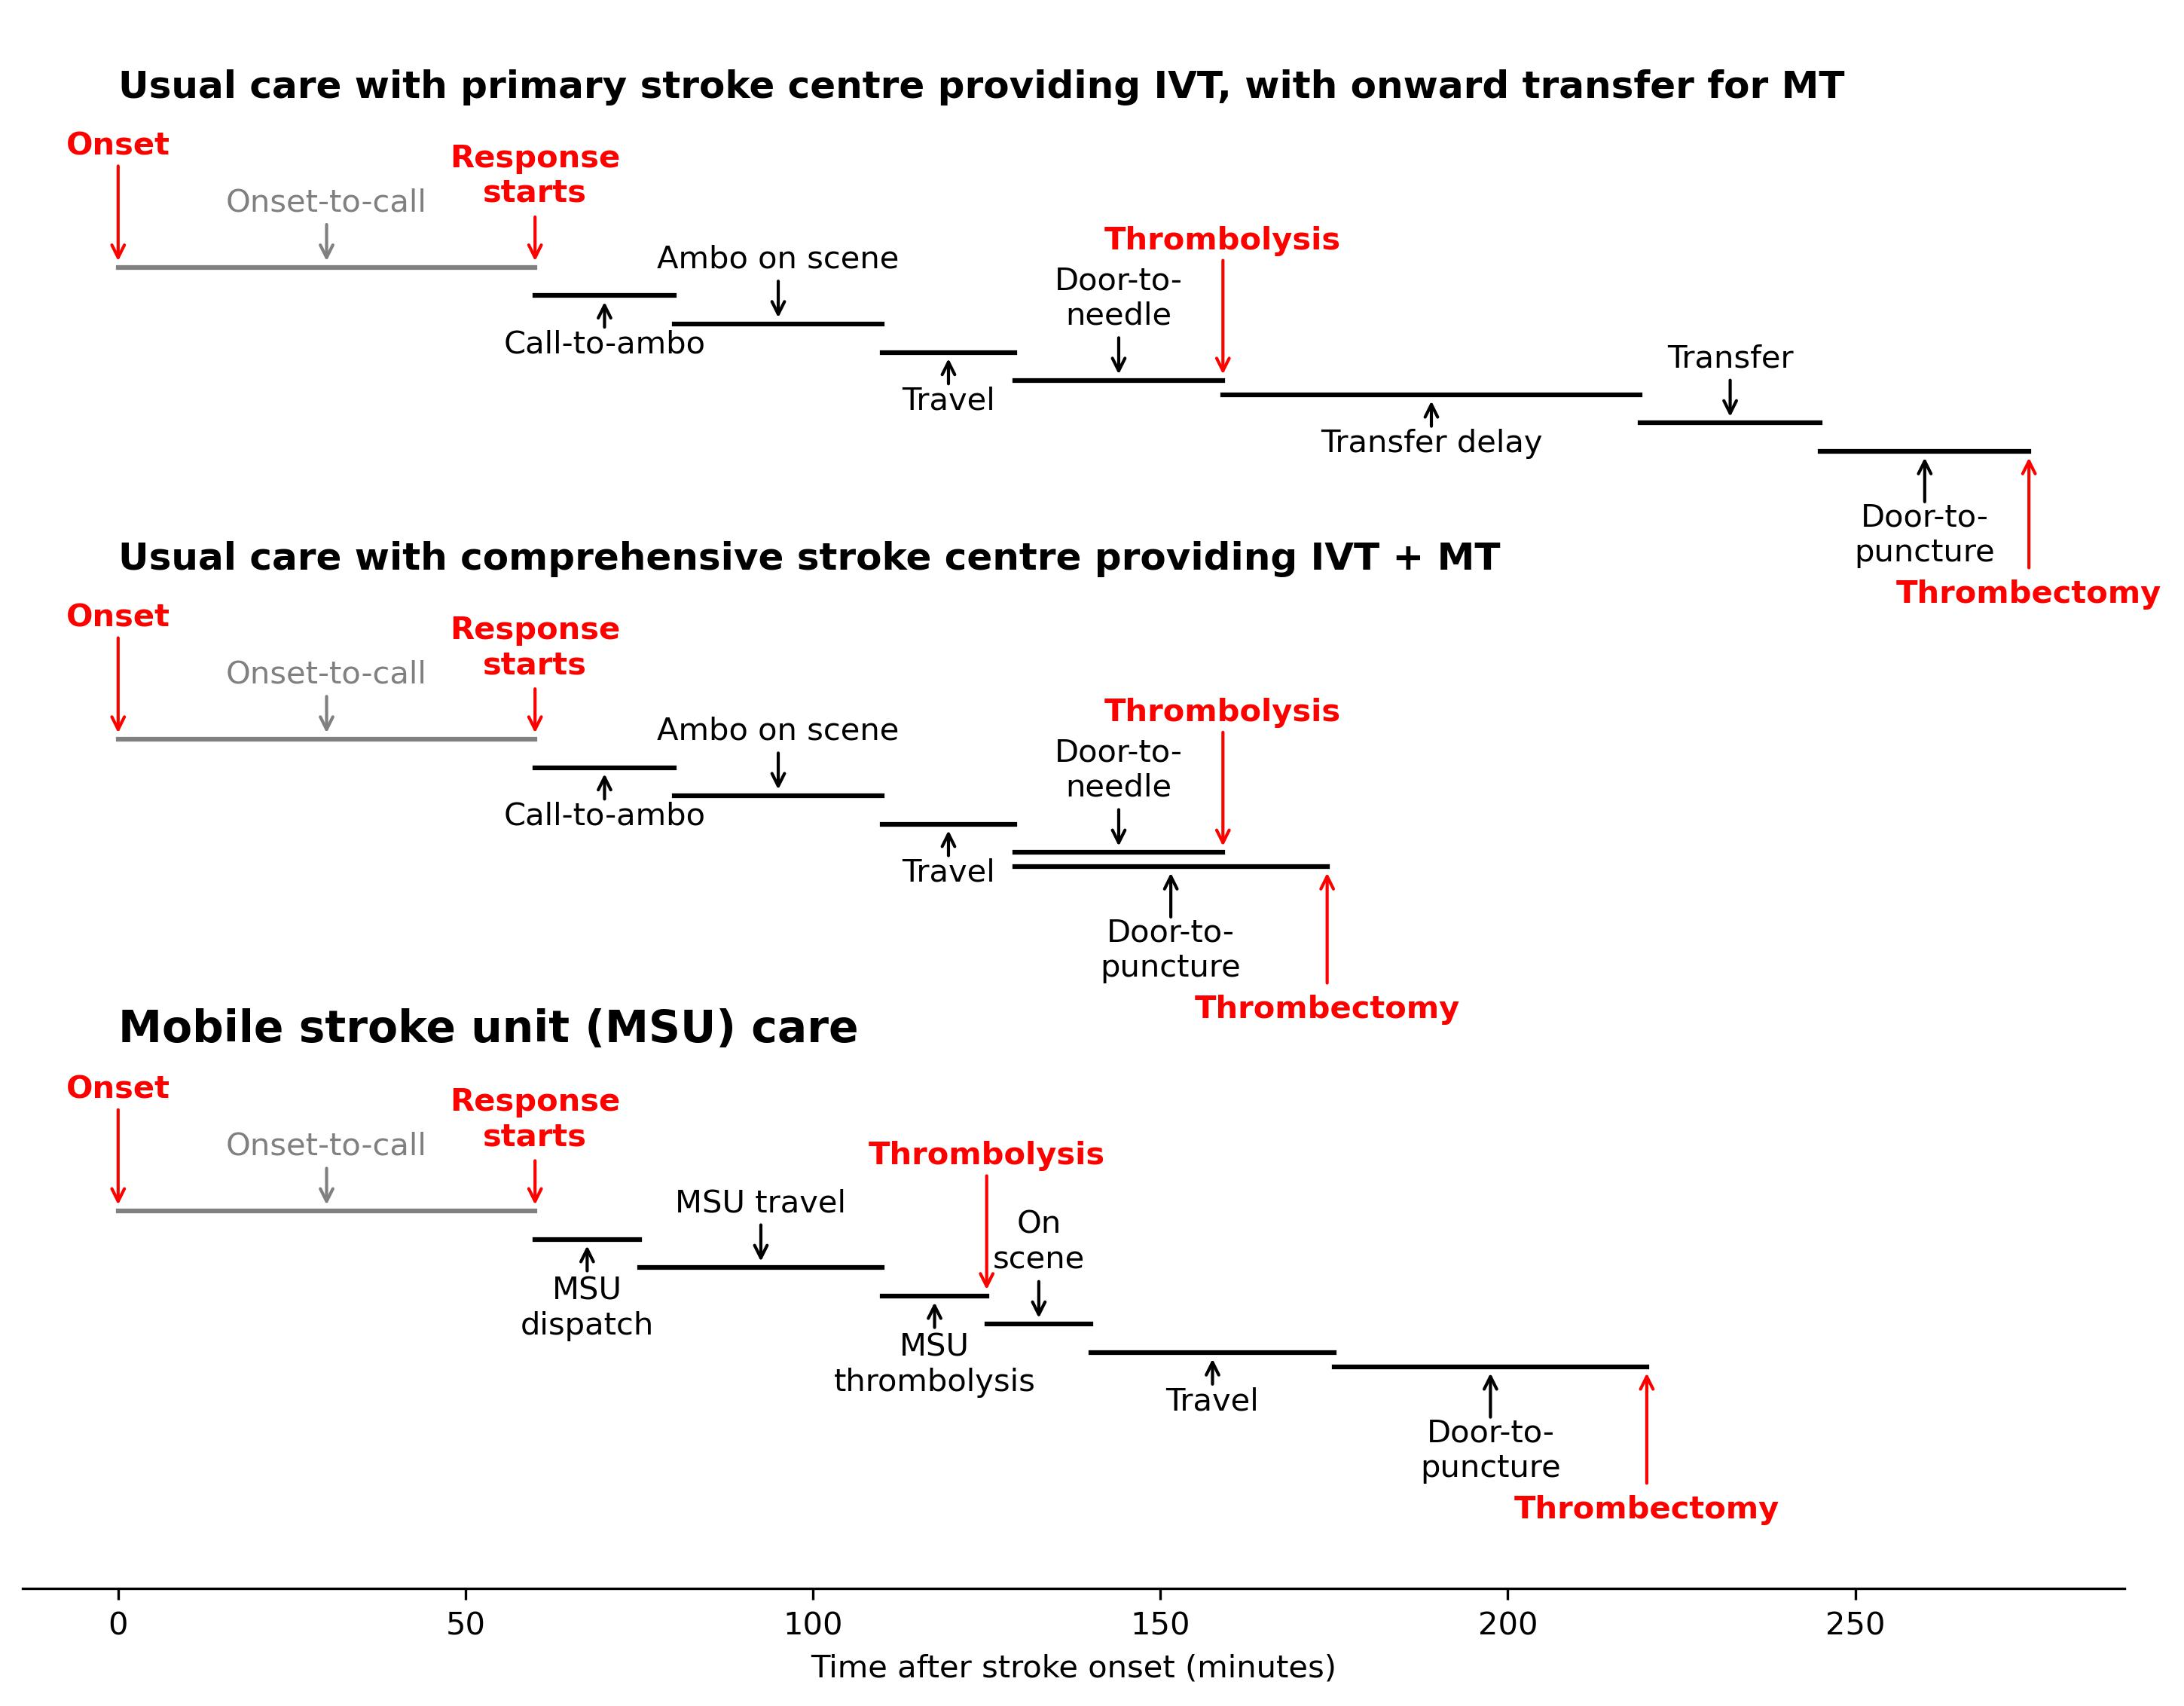
\includegraphics[width=0.85\linewidth]{images/stroke_treatment.jpg}
    \caption{An illustrative timeline showing processes included in the three pathways that are modelled for provision of IVT and MT. Top: Usual care pathway for patients with a PSC closest to their home LSOA, with the PSC providing IVT, followed by the LVO patients having a transfer to the nearest CSC for MT. Middle: Usual care pathway for patients with a CSC closest to their home LSOA, with the CSC providing both IVT and MT. Bottom: MSU care pathway, with IVT provided on-scene by the MSU, followed by the MSU transferring the LVO patients to the nearest CSC for MT. Process times other than travel times are common for all patients (defined by the scenario). Travel times depend on locations of patient and hospitals, with results calculated for all LSOAs in England.}
    \label{fig:process}
\end{figure}

\begin{figure}[h!]
    \centering
    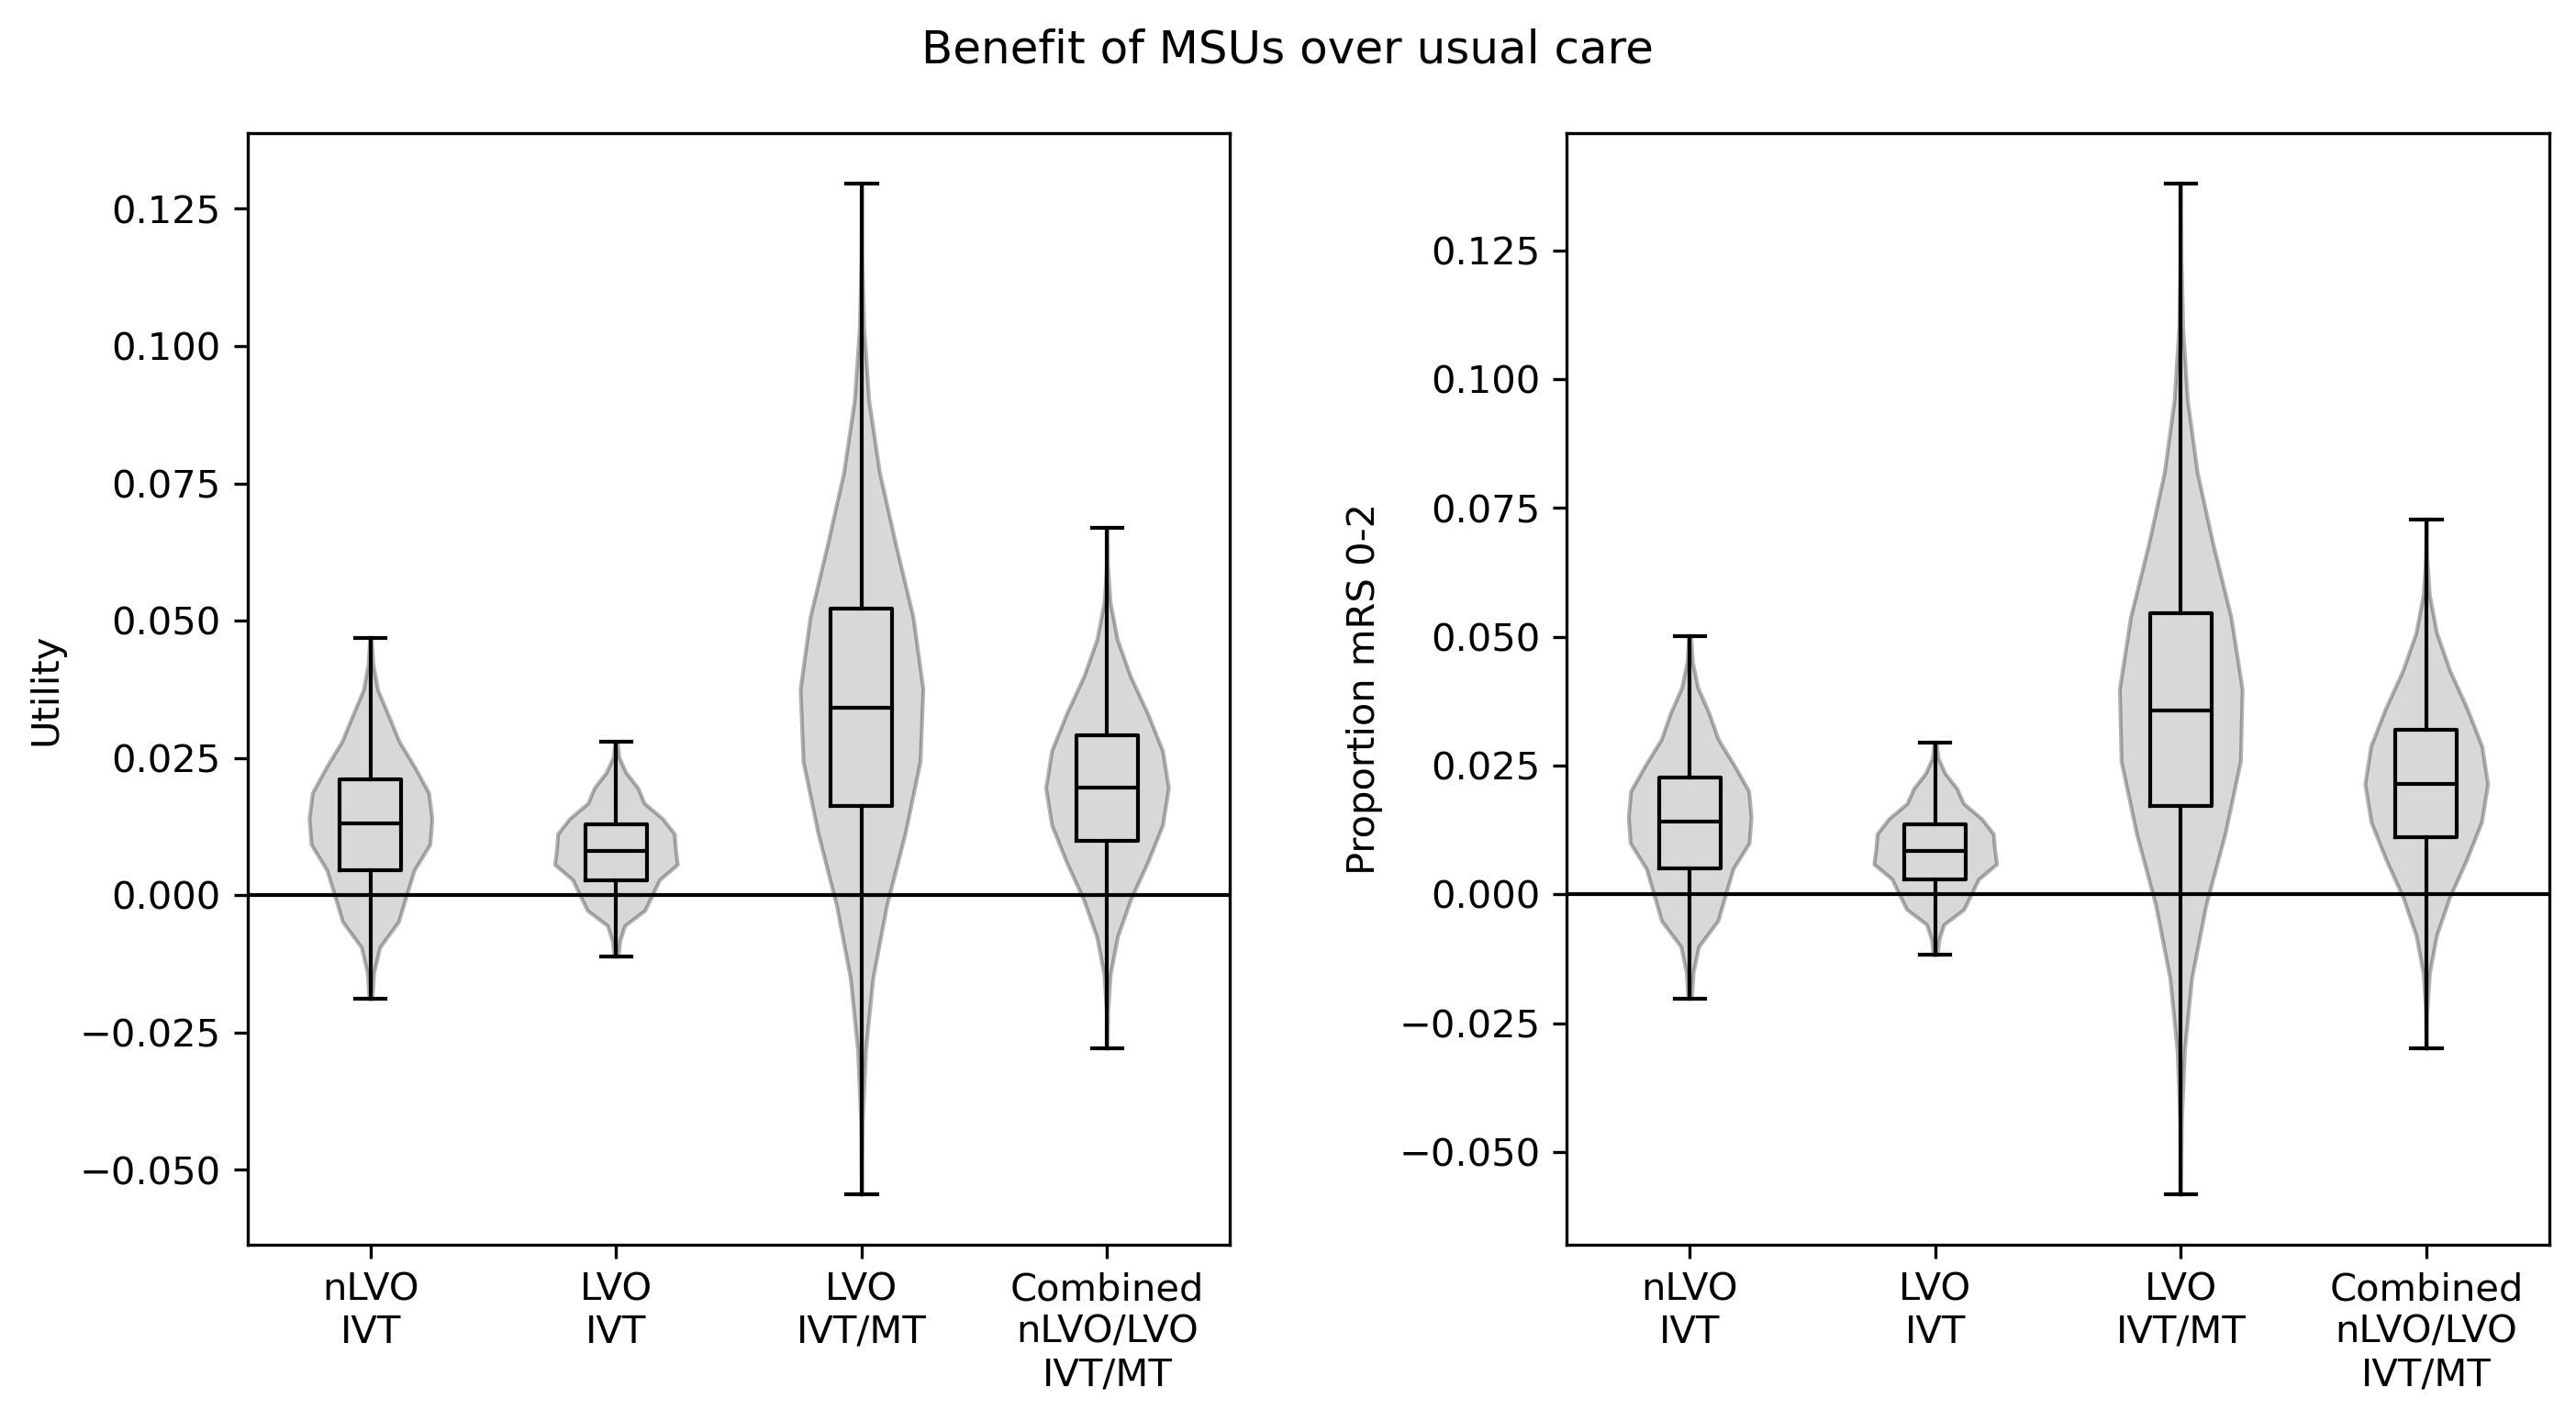
\includegraphics[width=0.75\linewidth]{images/scenario_results_summary.png}
    \caption{Benefit of MSU care over usual care across all scenarios (exploring the effect of changing process durations), in the treated population, measured by utility (left) or the proportion of patients with an outcome of mRS 0-2 (right), separating the changes for patients with nLVO and LVO. Results for LVO patients show the effect of MSU care on the benefit derived from IVT alone, or by IVT/MT in combination. Box plots show range, interquartile range, and median across all scenarios. The combined nLVO/LVO benefit assumed 70\% nLVO and 30\% LVO in the treated population, with LVOs receiving IVT/MT in combination. Overlaid over the box plots are violin plots showing the distribution of results across all scenarios. A positive value indicates MSU care provides an advantage over usual care, and a negative value indicates MSU care is disadvantageous compared with usual care. Results are the average effect across all LSOAs in England.}
    \label{fig:scenarios_overview}
    
\end{figure}
\begin{figure}[h!]
    \centering
    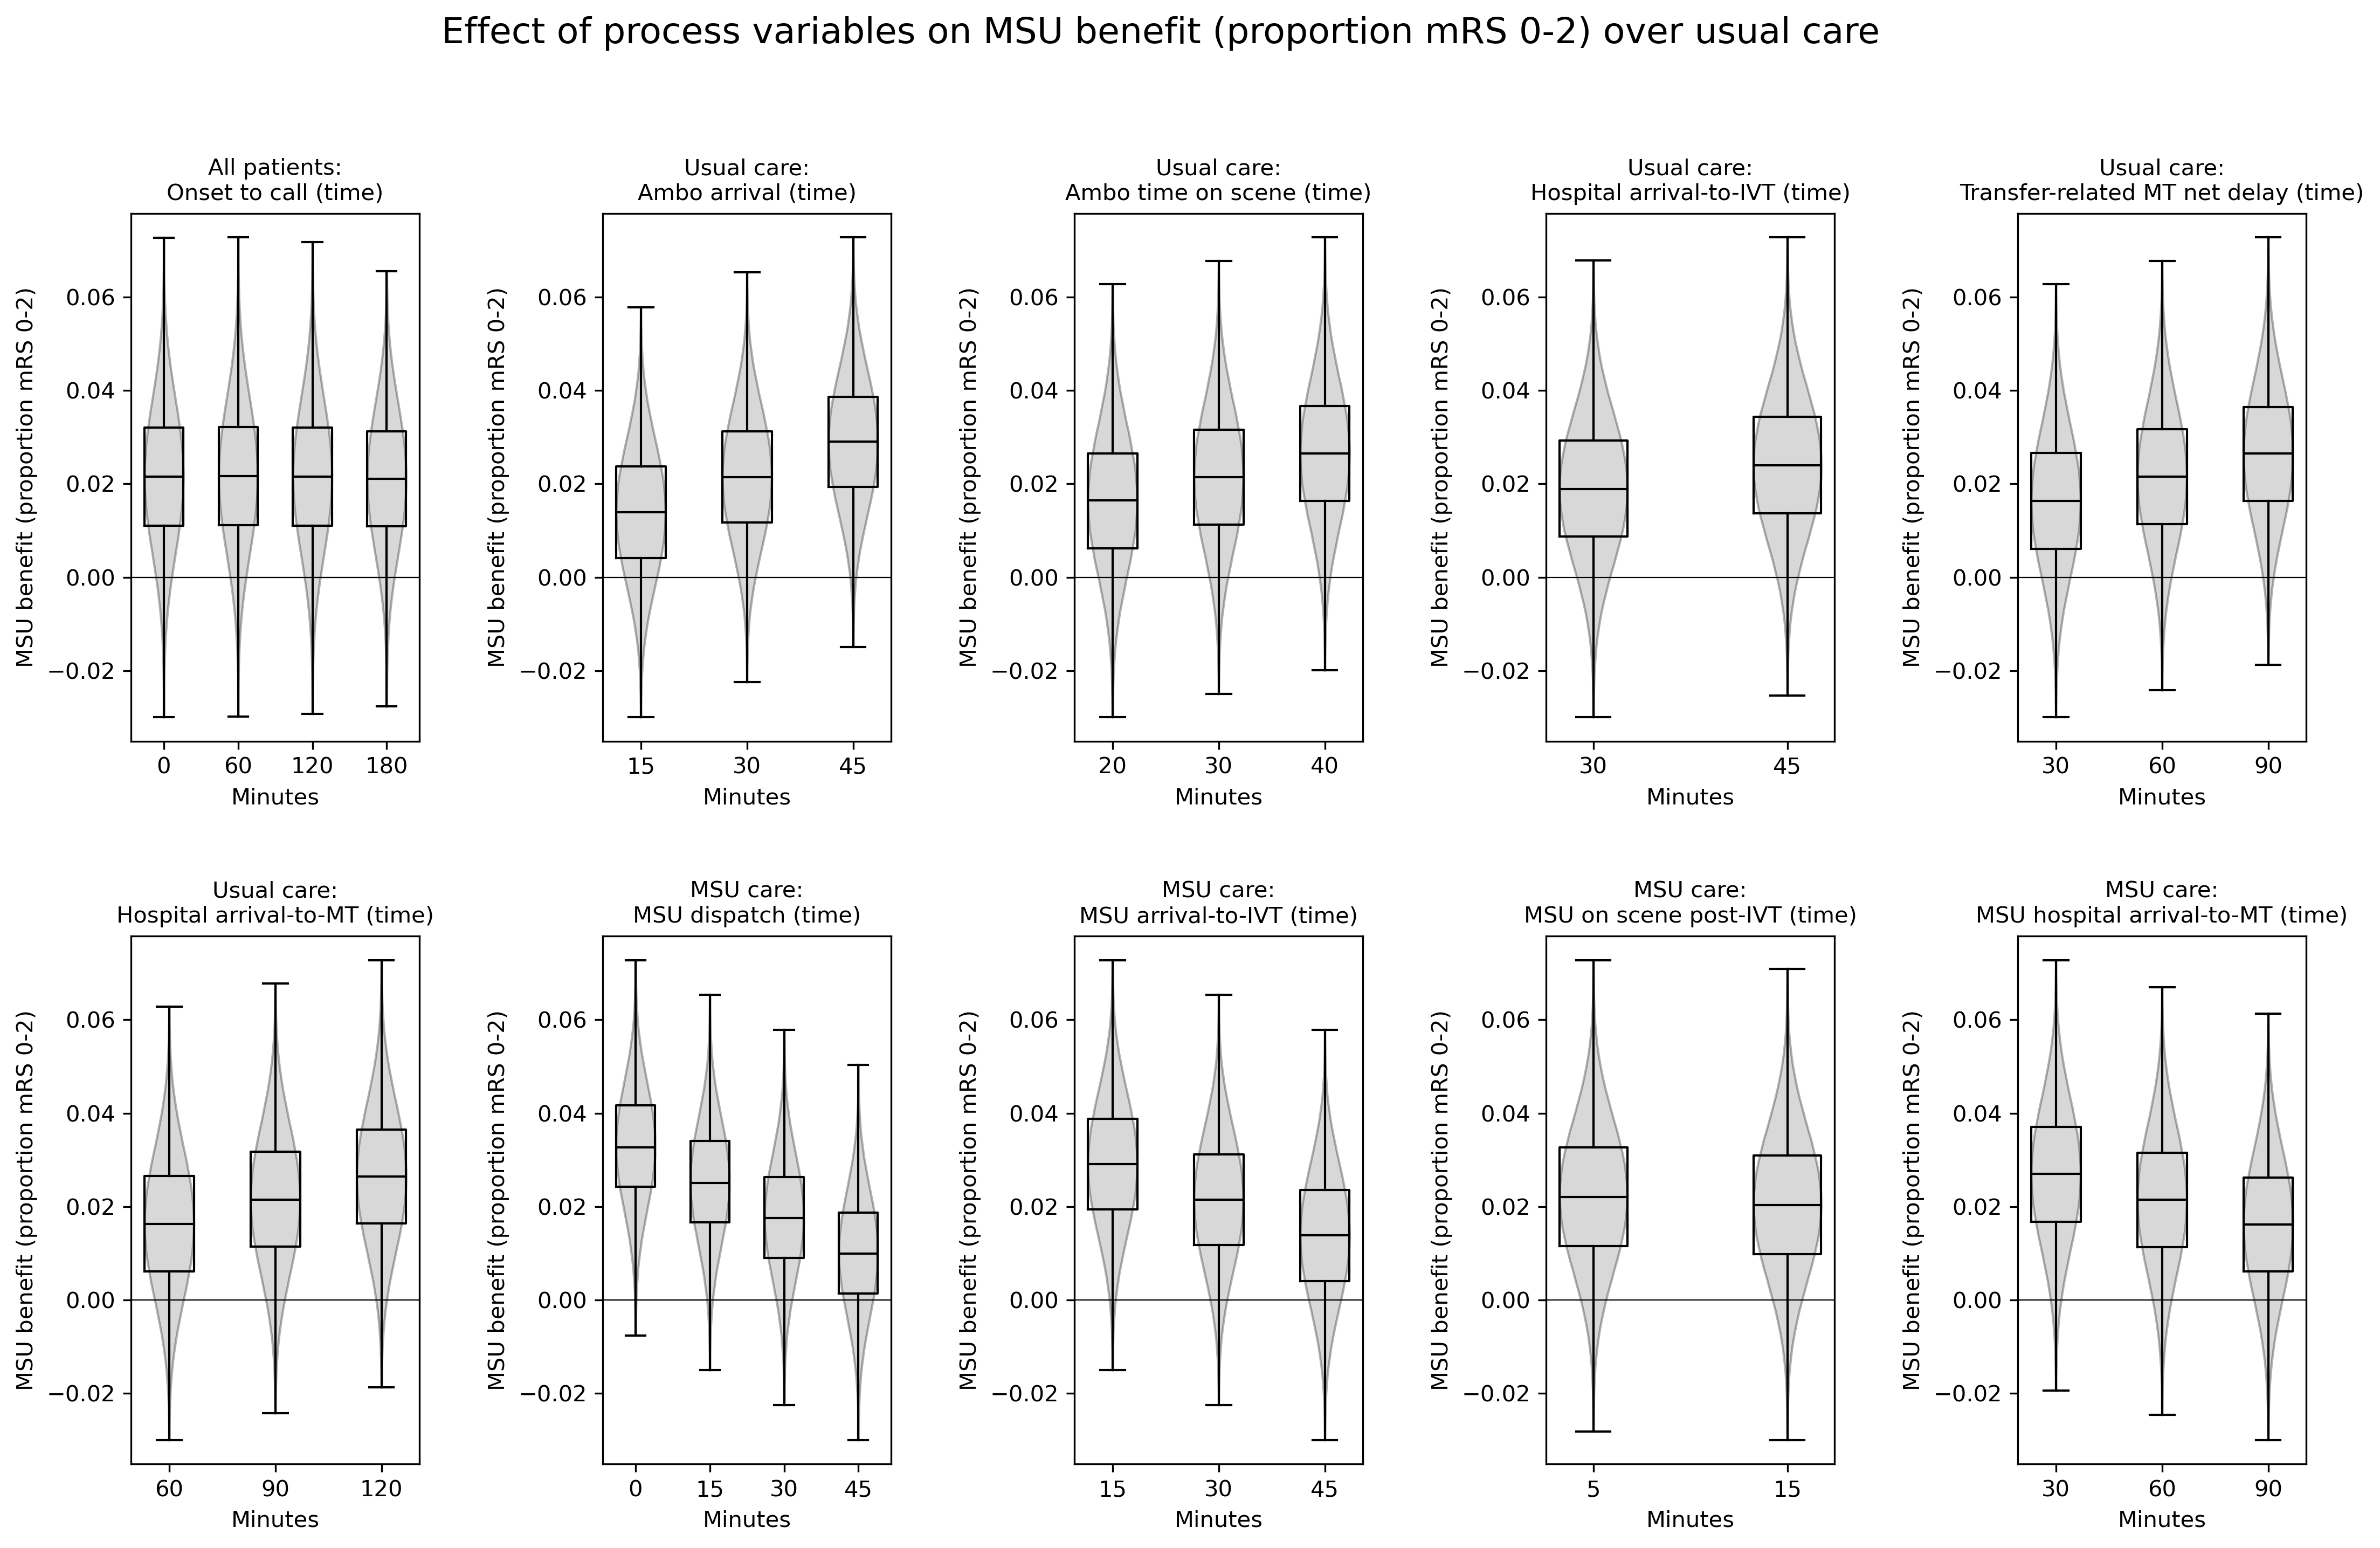
\includegraphics[width=1\linewidth]{images/msu_net_mrs_0-2_benefit.png}
    \caption{The effect of changing modelled process durations on the predicted benefit of MSU care over usual care, in the treated population (comprised of 30\% nLVO and 70\% LVO patients, where nLVO patients receive IVT and LVO patients receive IVT followed by MT), measured by proportion of patients with an outcome of mRS 0-2. For each target parameter, results are averaged across all scenarios with that given parameter value. Box plots show range, interquartile range, and median, across all scenarios. Overlaid over the box plots are violin plots showing the distribution of results across all scenarios. Results are the average effect across all LSOAs in England.}
    \label{fig:scenarios_mrs}
\end{figure}

\begin{figure}[h!]
    \centering
    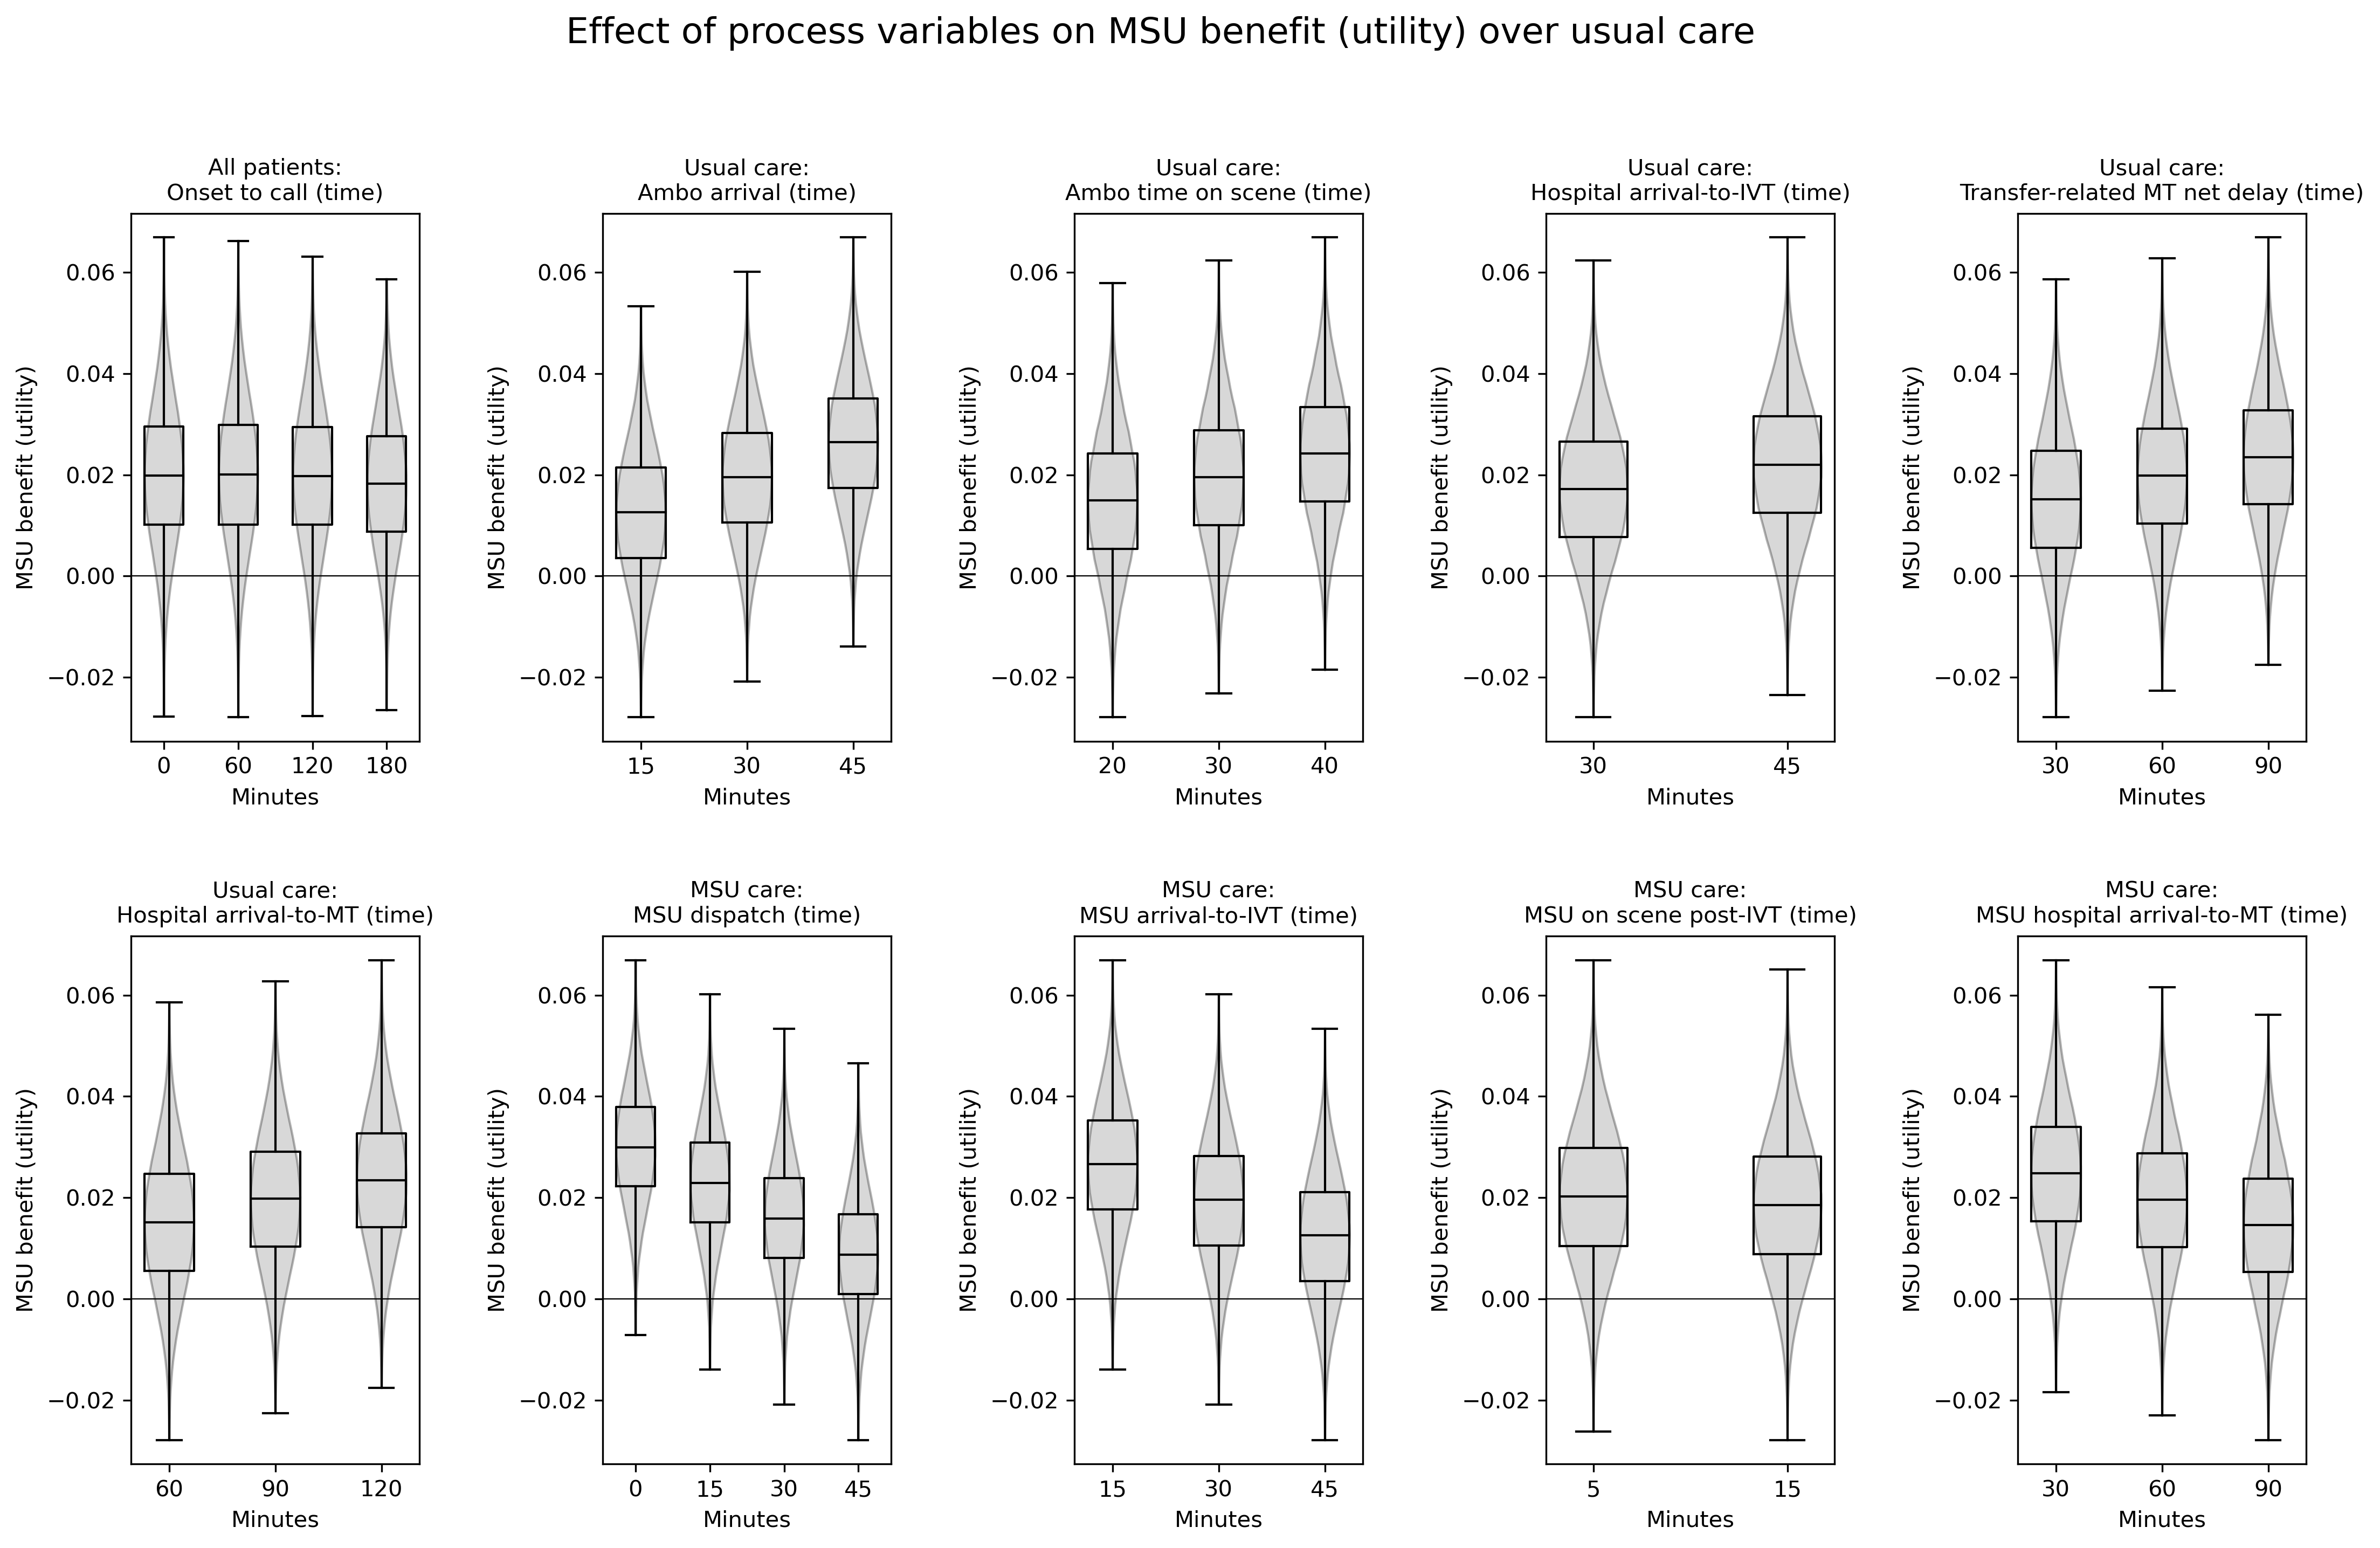
\includegraphics[width=1\linewidth]{images/msu_net_utility_benefit.png}
    \caption{The effect of changing modelled process durations on the predicted benefit of MSU care over usual care, in the treated population (comprised of 30\% nLVO and 70\% LVO patients, where nLVO patients receive IVT and LVO patients receive IVT followed by MT), measured by utility. For each target parameter, results are averaged across all scenarios with that given parameter value. Box plots show range, interquartile range, and median, across all scenarios. Overlaid over the box plots are violin plots showing the distribution of results across all scenarios. Results are the average effect across all LSOAs in England.}
    \label{fig:scenarios_utility}
\end{figure}

\begin{figure}[h!]
    \centering
    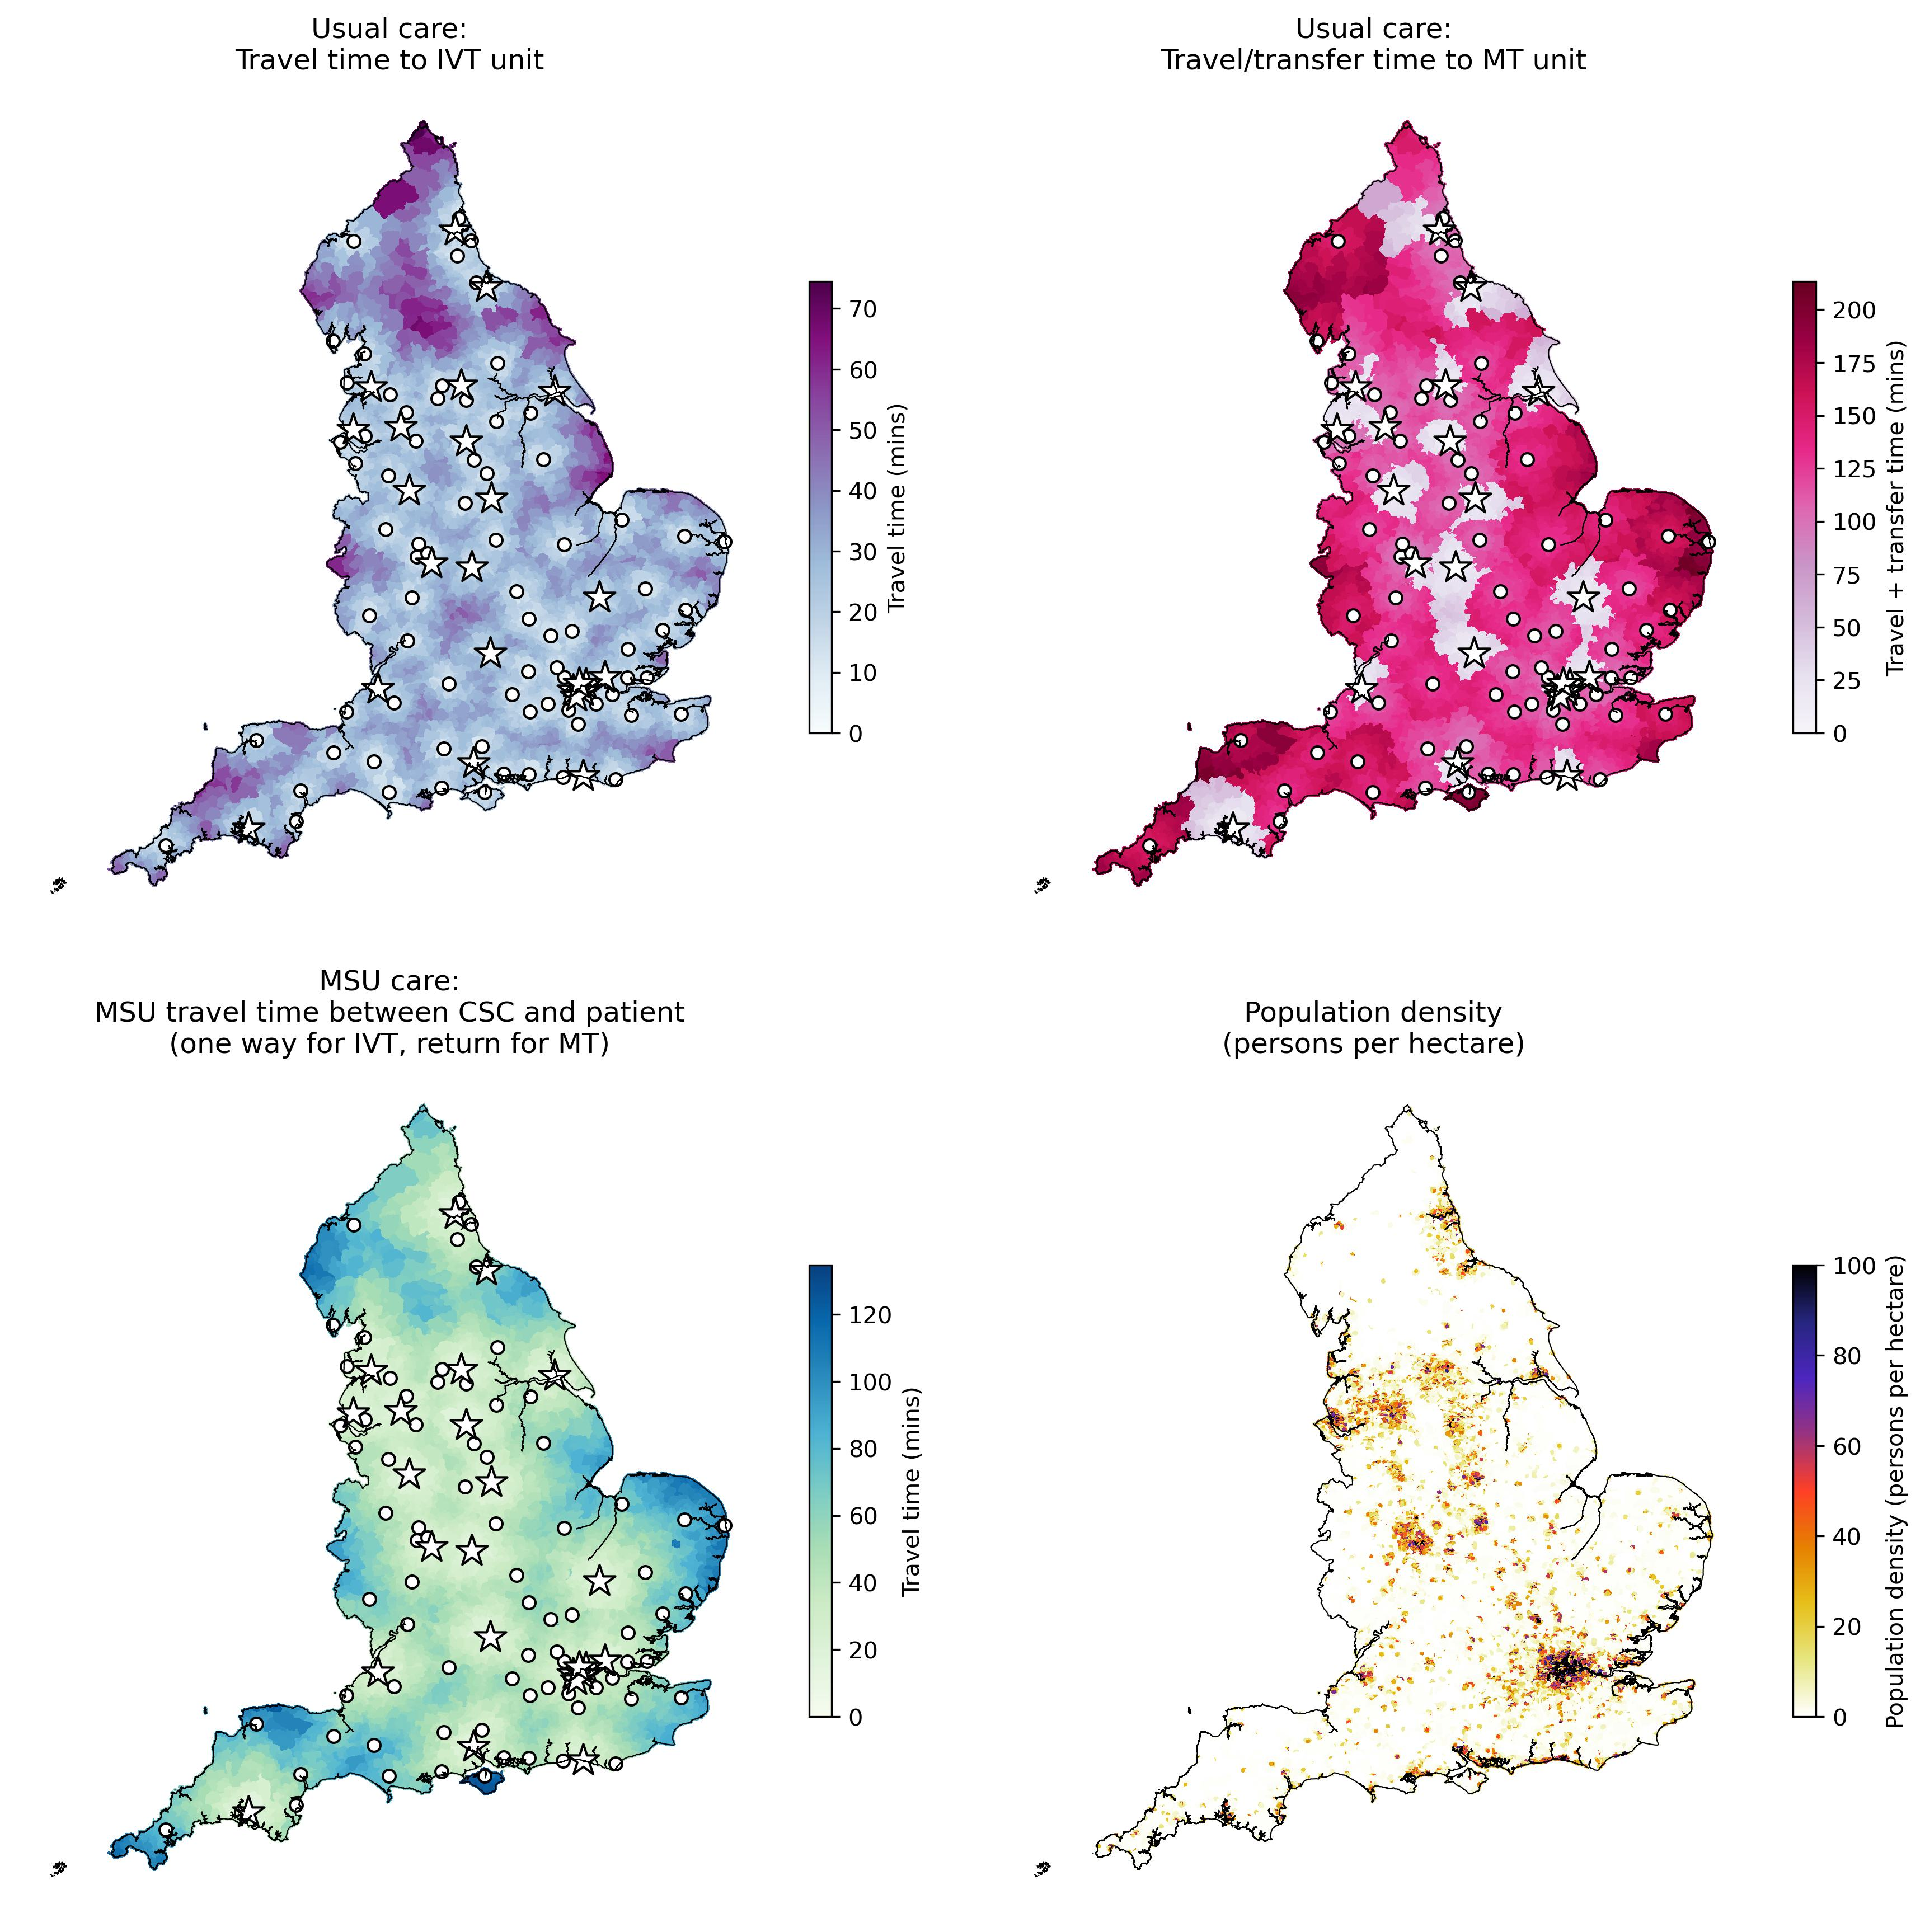
\includegraphics[width=1.0\linewidth]{images/map_times.jpg}
    \caption{Travel times to treatment under the two treatment delivery models, and population density for each LSOA. \textit{Top left}: With \emph{usual care} the travel times from the patients LSOA to their nearest PSC (providing only IVT). \textit{Top right}: With \emph{usual care} the travel and, where necessary, transfer times from the patients LSOA to a CSC (providing MT). For those patients that first attend a PSC providing only IVT, the times shown include the travel time to the PSC, a net additional delay of 60 minutes, and the inter-hospital travel time between PSC and CSC. \textit{Bottom left}: With \emph{MSU care} with the MSU base locations at the current 23 CSCs, the travel times for the MSU between the patients LSOA and their nearest CSC (one way for travel time to IVT, return journey for travel time to MT). \textit{Bottom right}: Population density (with scale capped at 100 persons per hectare). Circles show locations of PSCs (providing only IVT). Stars show locations of CSCs (providing both IVT and MT), and being the base locations of MSUs.}
    \label{fig:map_times}
\end{figure}

\begin{figure}[h!]
    \centering
    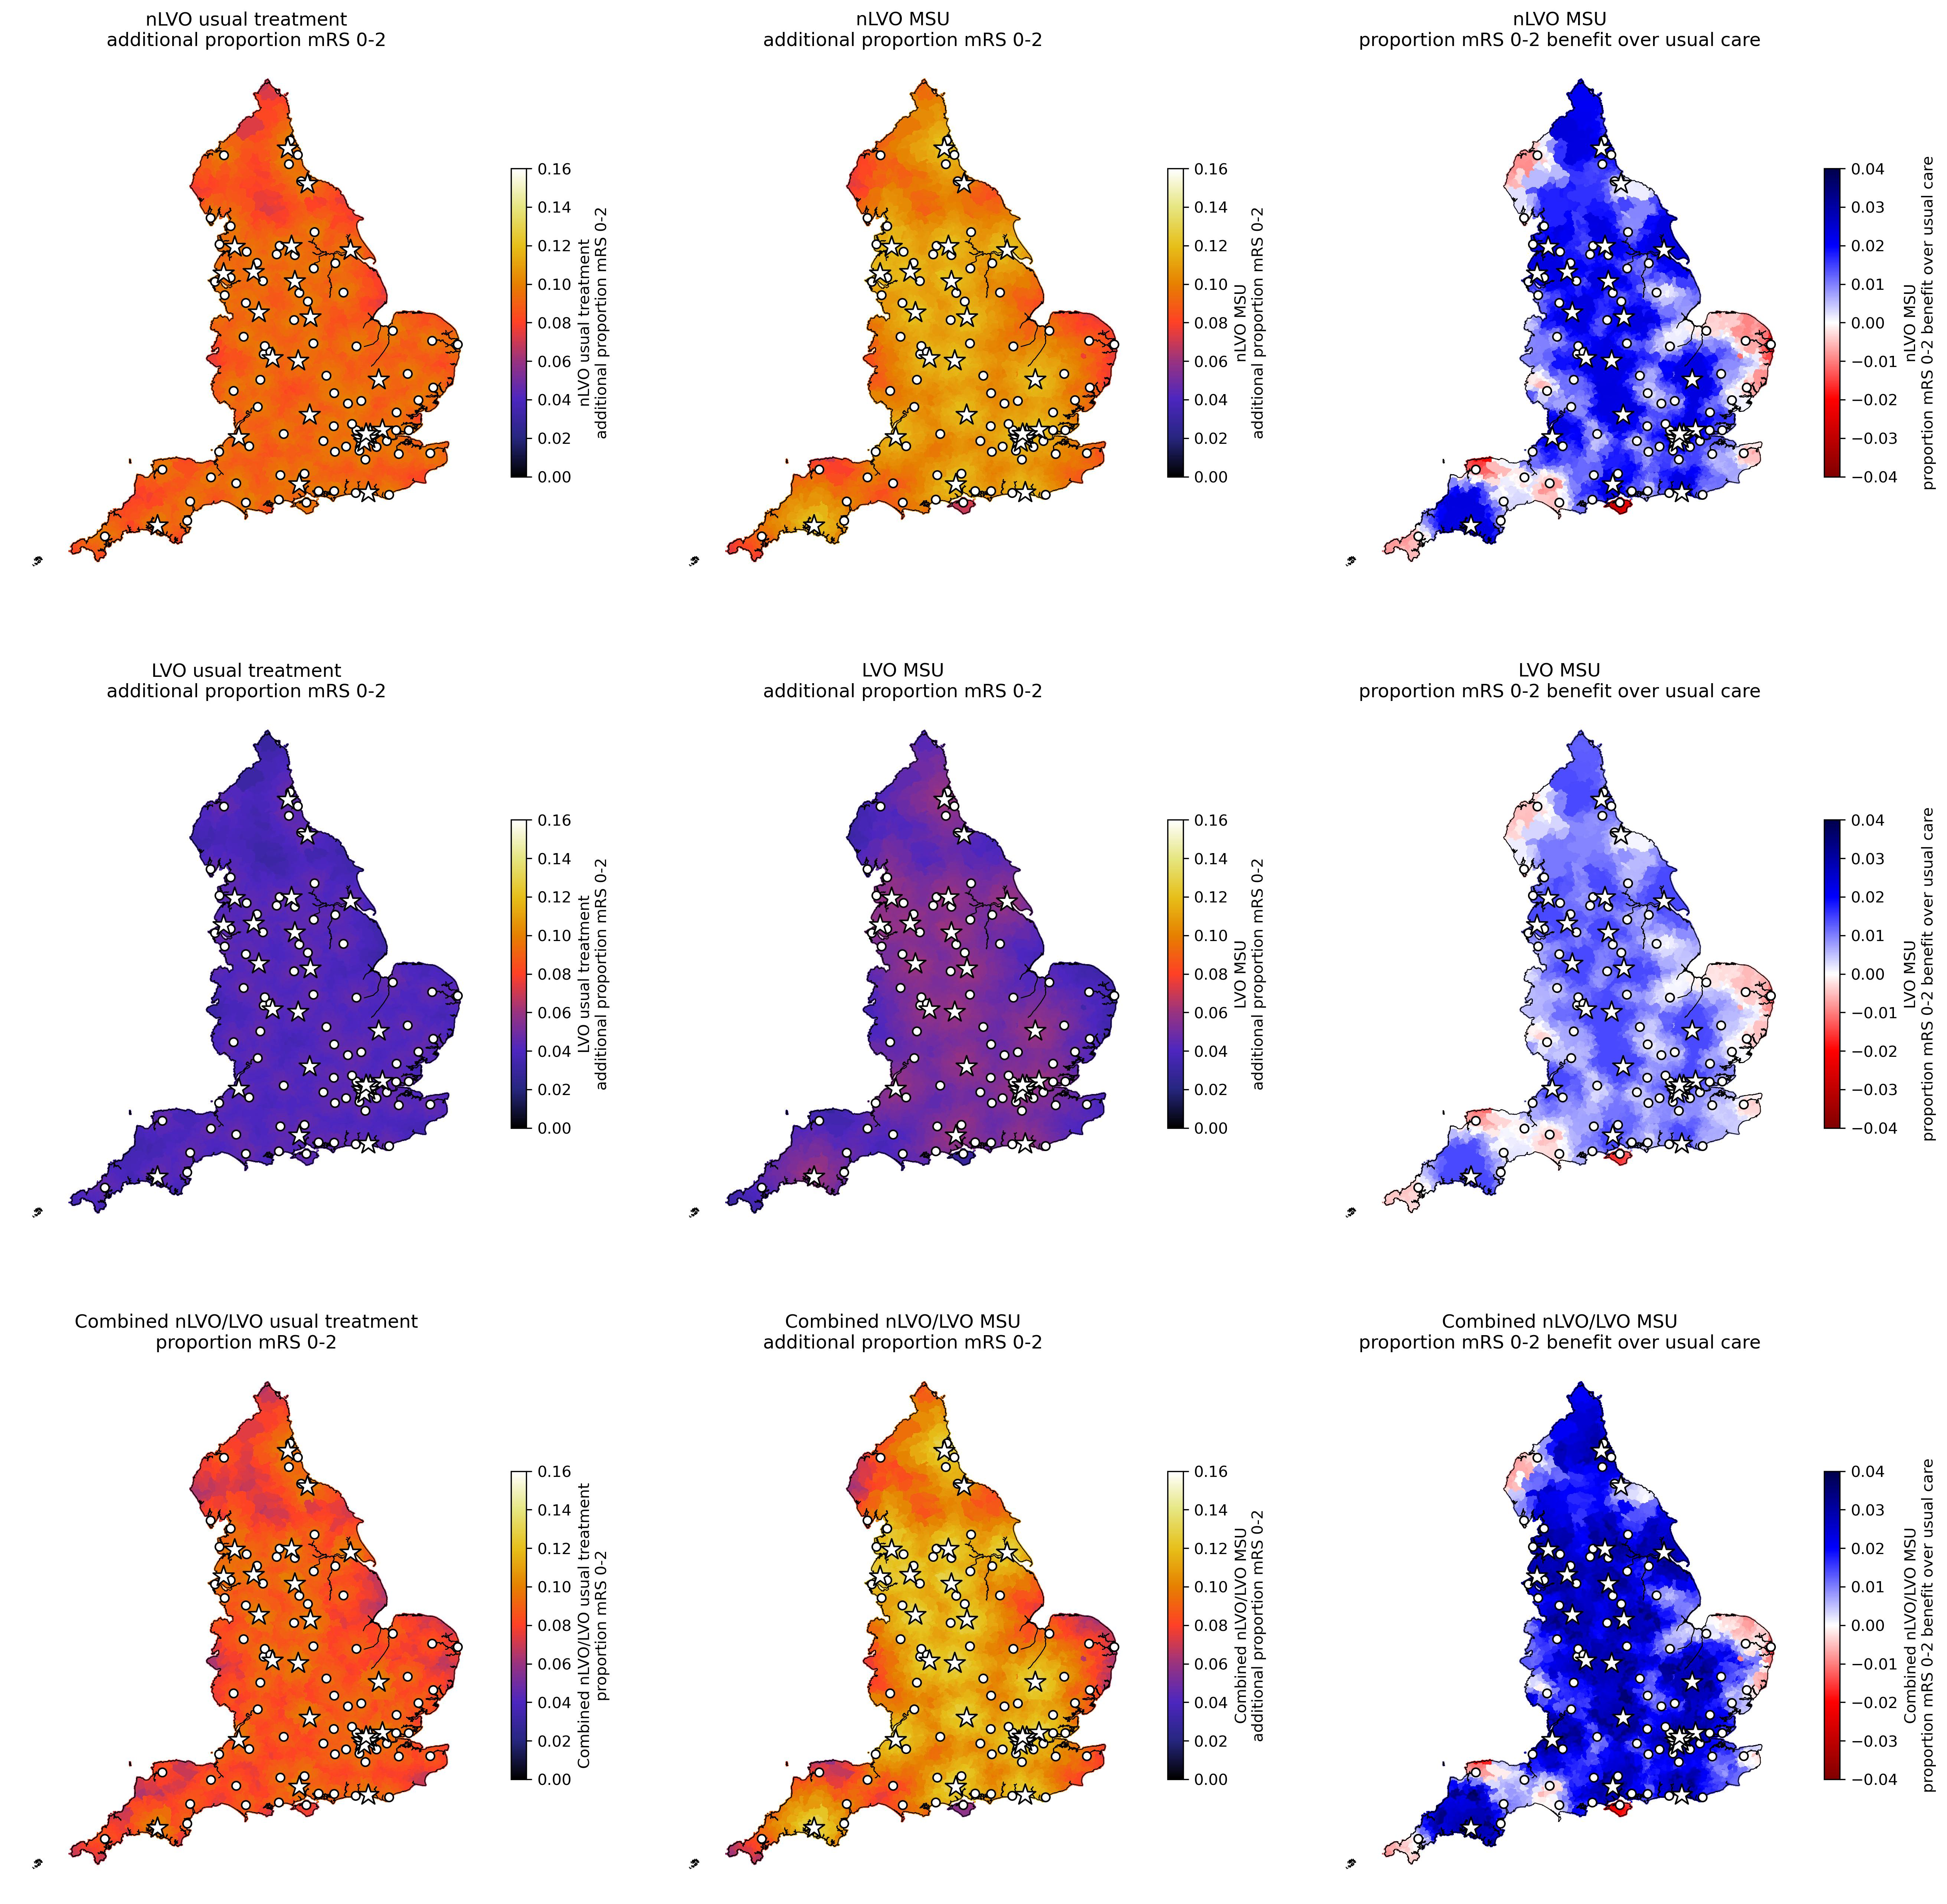
\includegraphics[width=1\linewidth]{images/map_mrs_0_2.jpg}
    \caption{Map of treatment benefits expressed as the proportion of patients with an outcome of mRS 0-2, calculated by LSOA for the treated population. \textit{Top}: Treatment of nLVO; \textit{Middle}: Treatment of LVO, \textit{Bottom}: Combination of treatment (based on 70\% nLVO and 30\% LVO in the treated population, with LVO receiving IVT/MT in combination). \textit{Left}: Benefit of usual care over no treatment; \textit{Middle}: Benefit of MSU care over no treatment; \textit{Right}: Benefit of MSU care over usual care. Circles show locations of PSCs (providing only IVT). Stars show locations of CSCs (providing both IVT and MT, and are also the base locations of MSUs).}
    \label{fig:msu_map_mrs_0_2}
\end{figure}

\begin{figure}[h!]
    \centering
    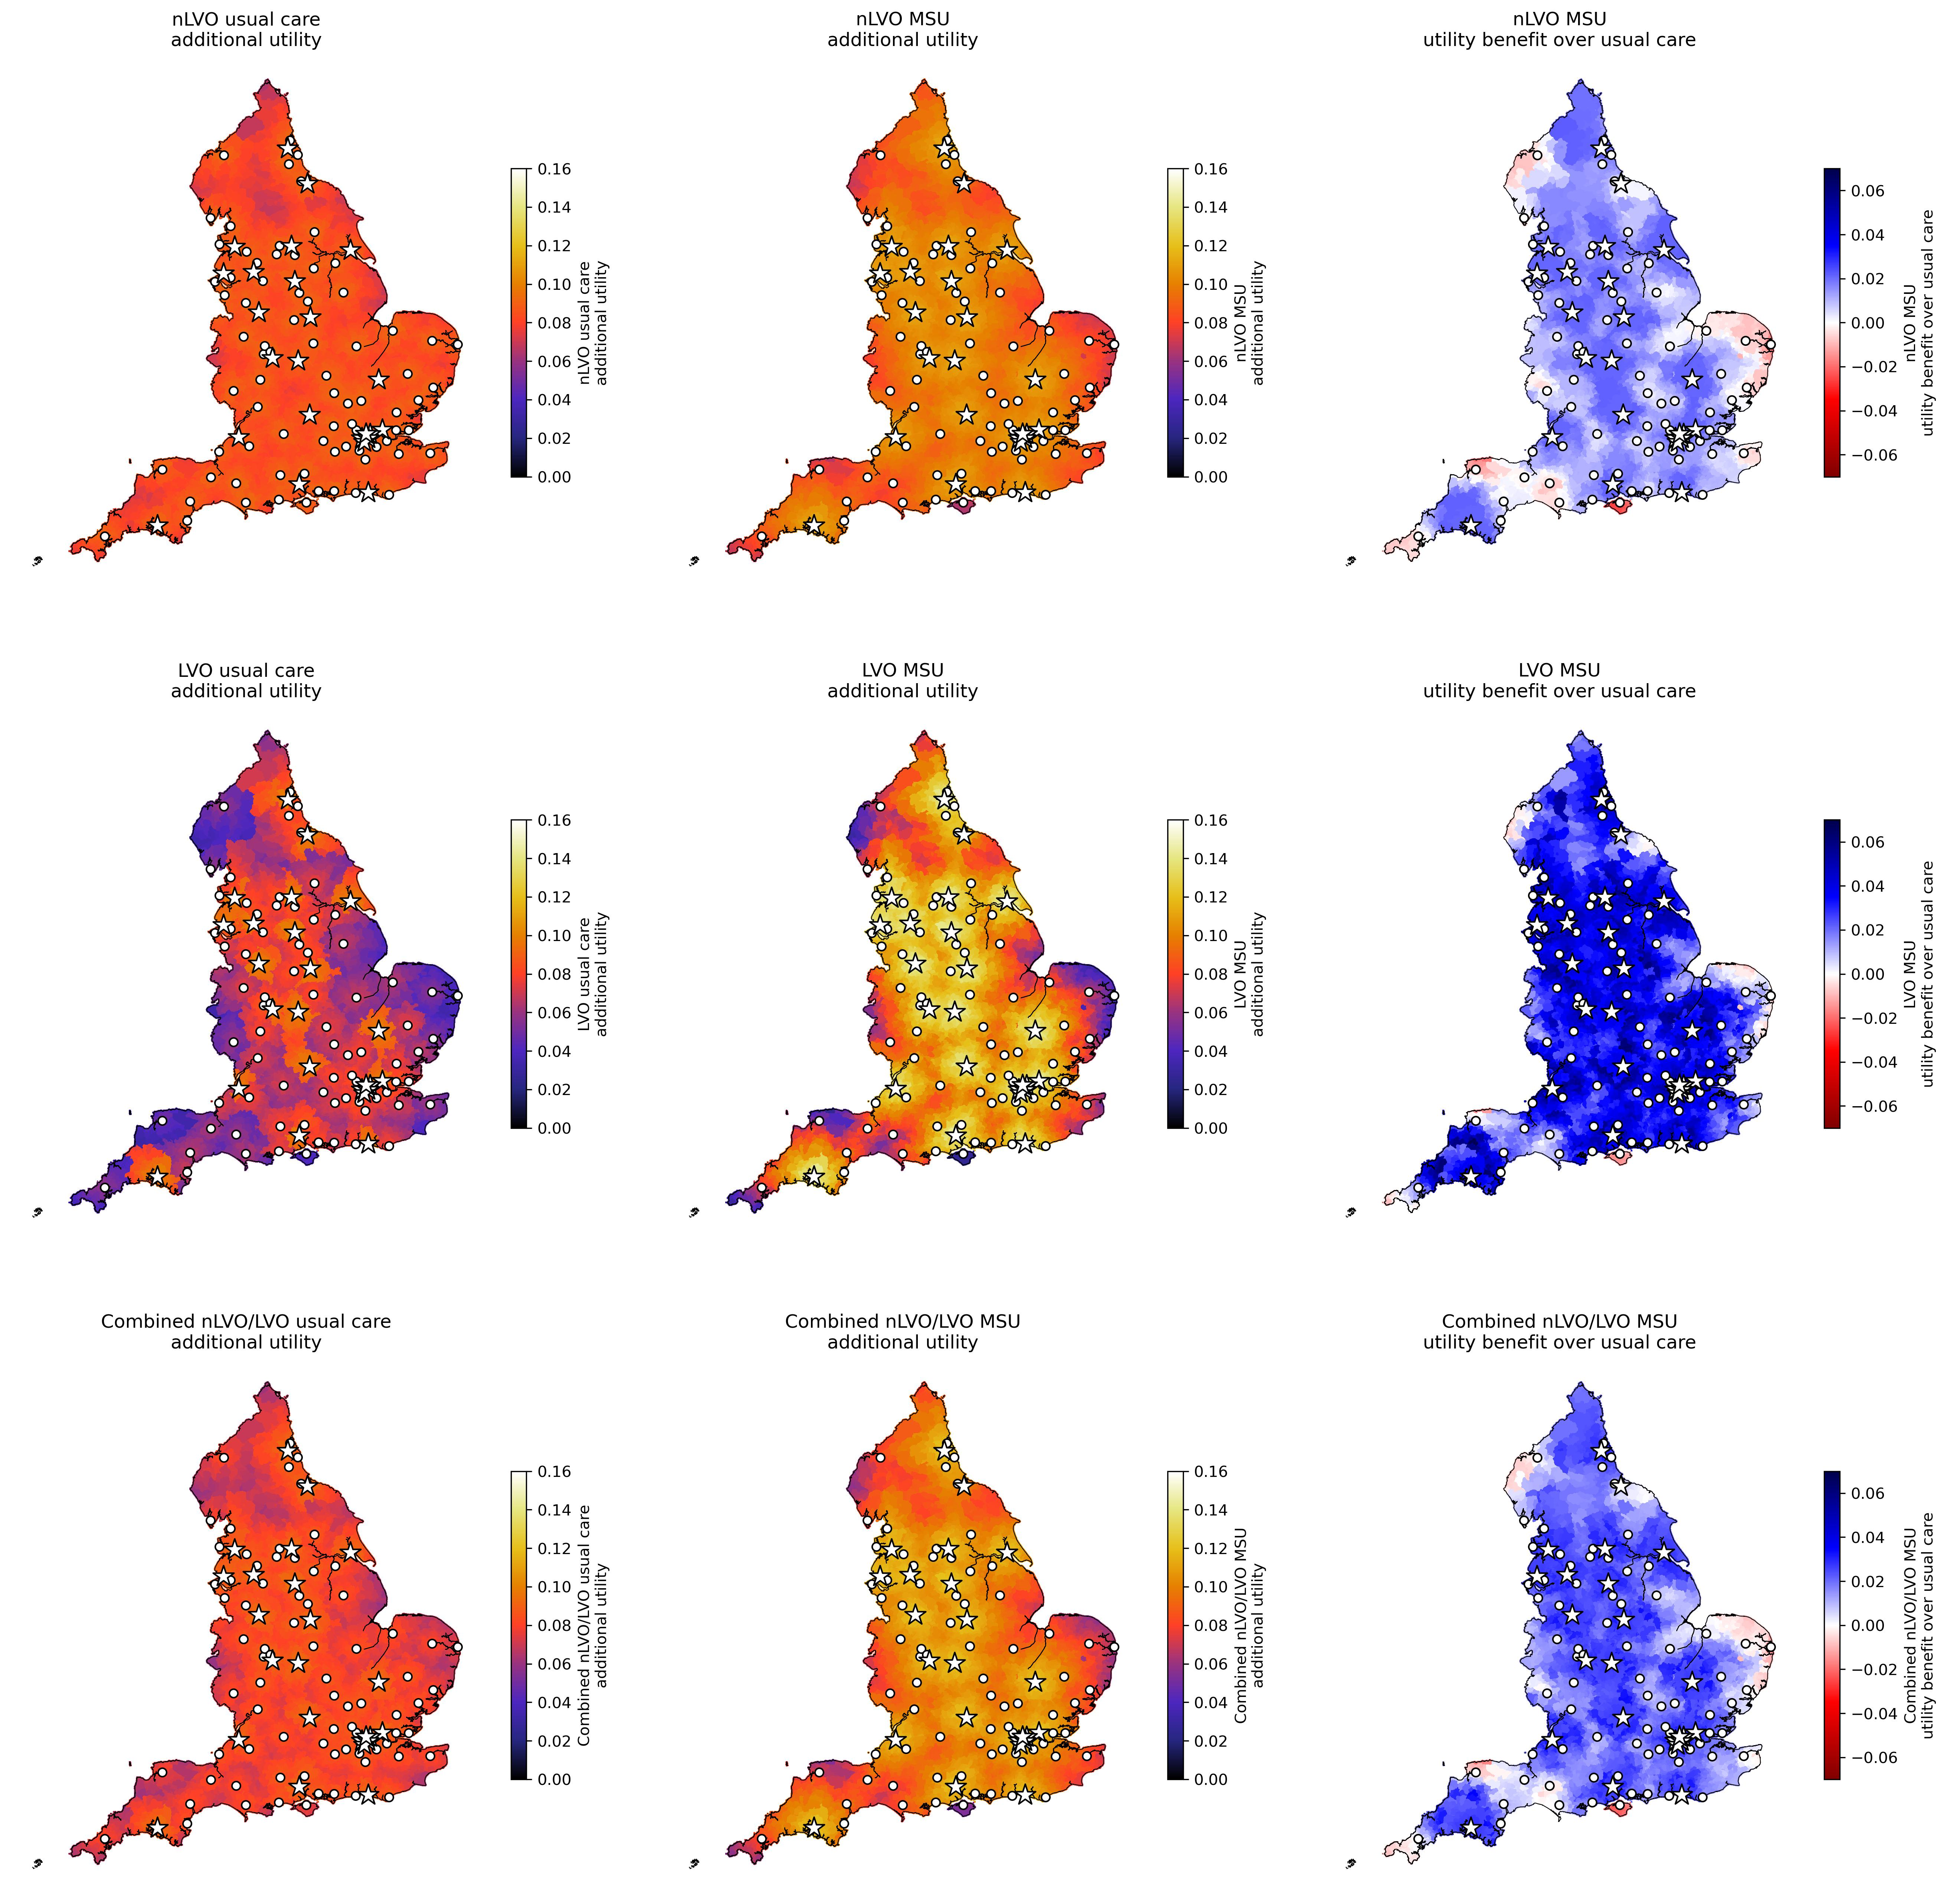
\includegraphics[width=1\linewidth]{images/map_utility.jpg}
    \caption{Map of treatment benefits expressed as the  utility benefit, calculated by LSOA for the treated population. \textit{Top}: Treatment of nLVO; \textit{Middle}: Treatment of LVO, \textit{Bottom}: Combination of treatment (based on 70\% nLVO and 30\% LVO in the treated population, with LVO receiving IVT/MT in combination). \textit{Left}: Benefit of usual care over no treatment; \textit{Middle}: Benefit of MSU care over no treatment; \textit{Right}: Benefit of MSU care over usual care. Circles show locations of PSCs (providing only IVT). Stars show locations of CSCs (providing both IVT and MT, and are also the base locations of MSUs).}
    \label{fig:msu_map_utility}
\end{figure}

\begin{figure}[h]
    \centering
    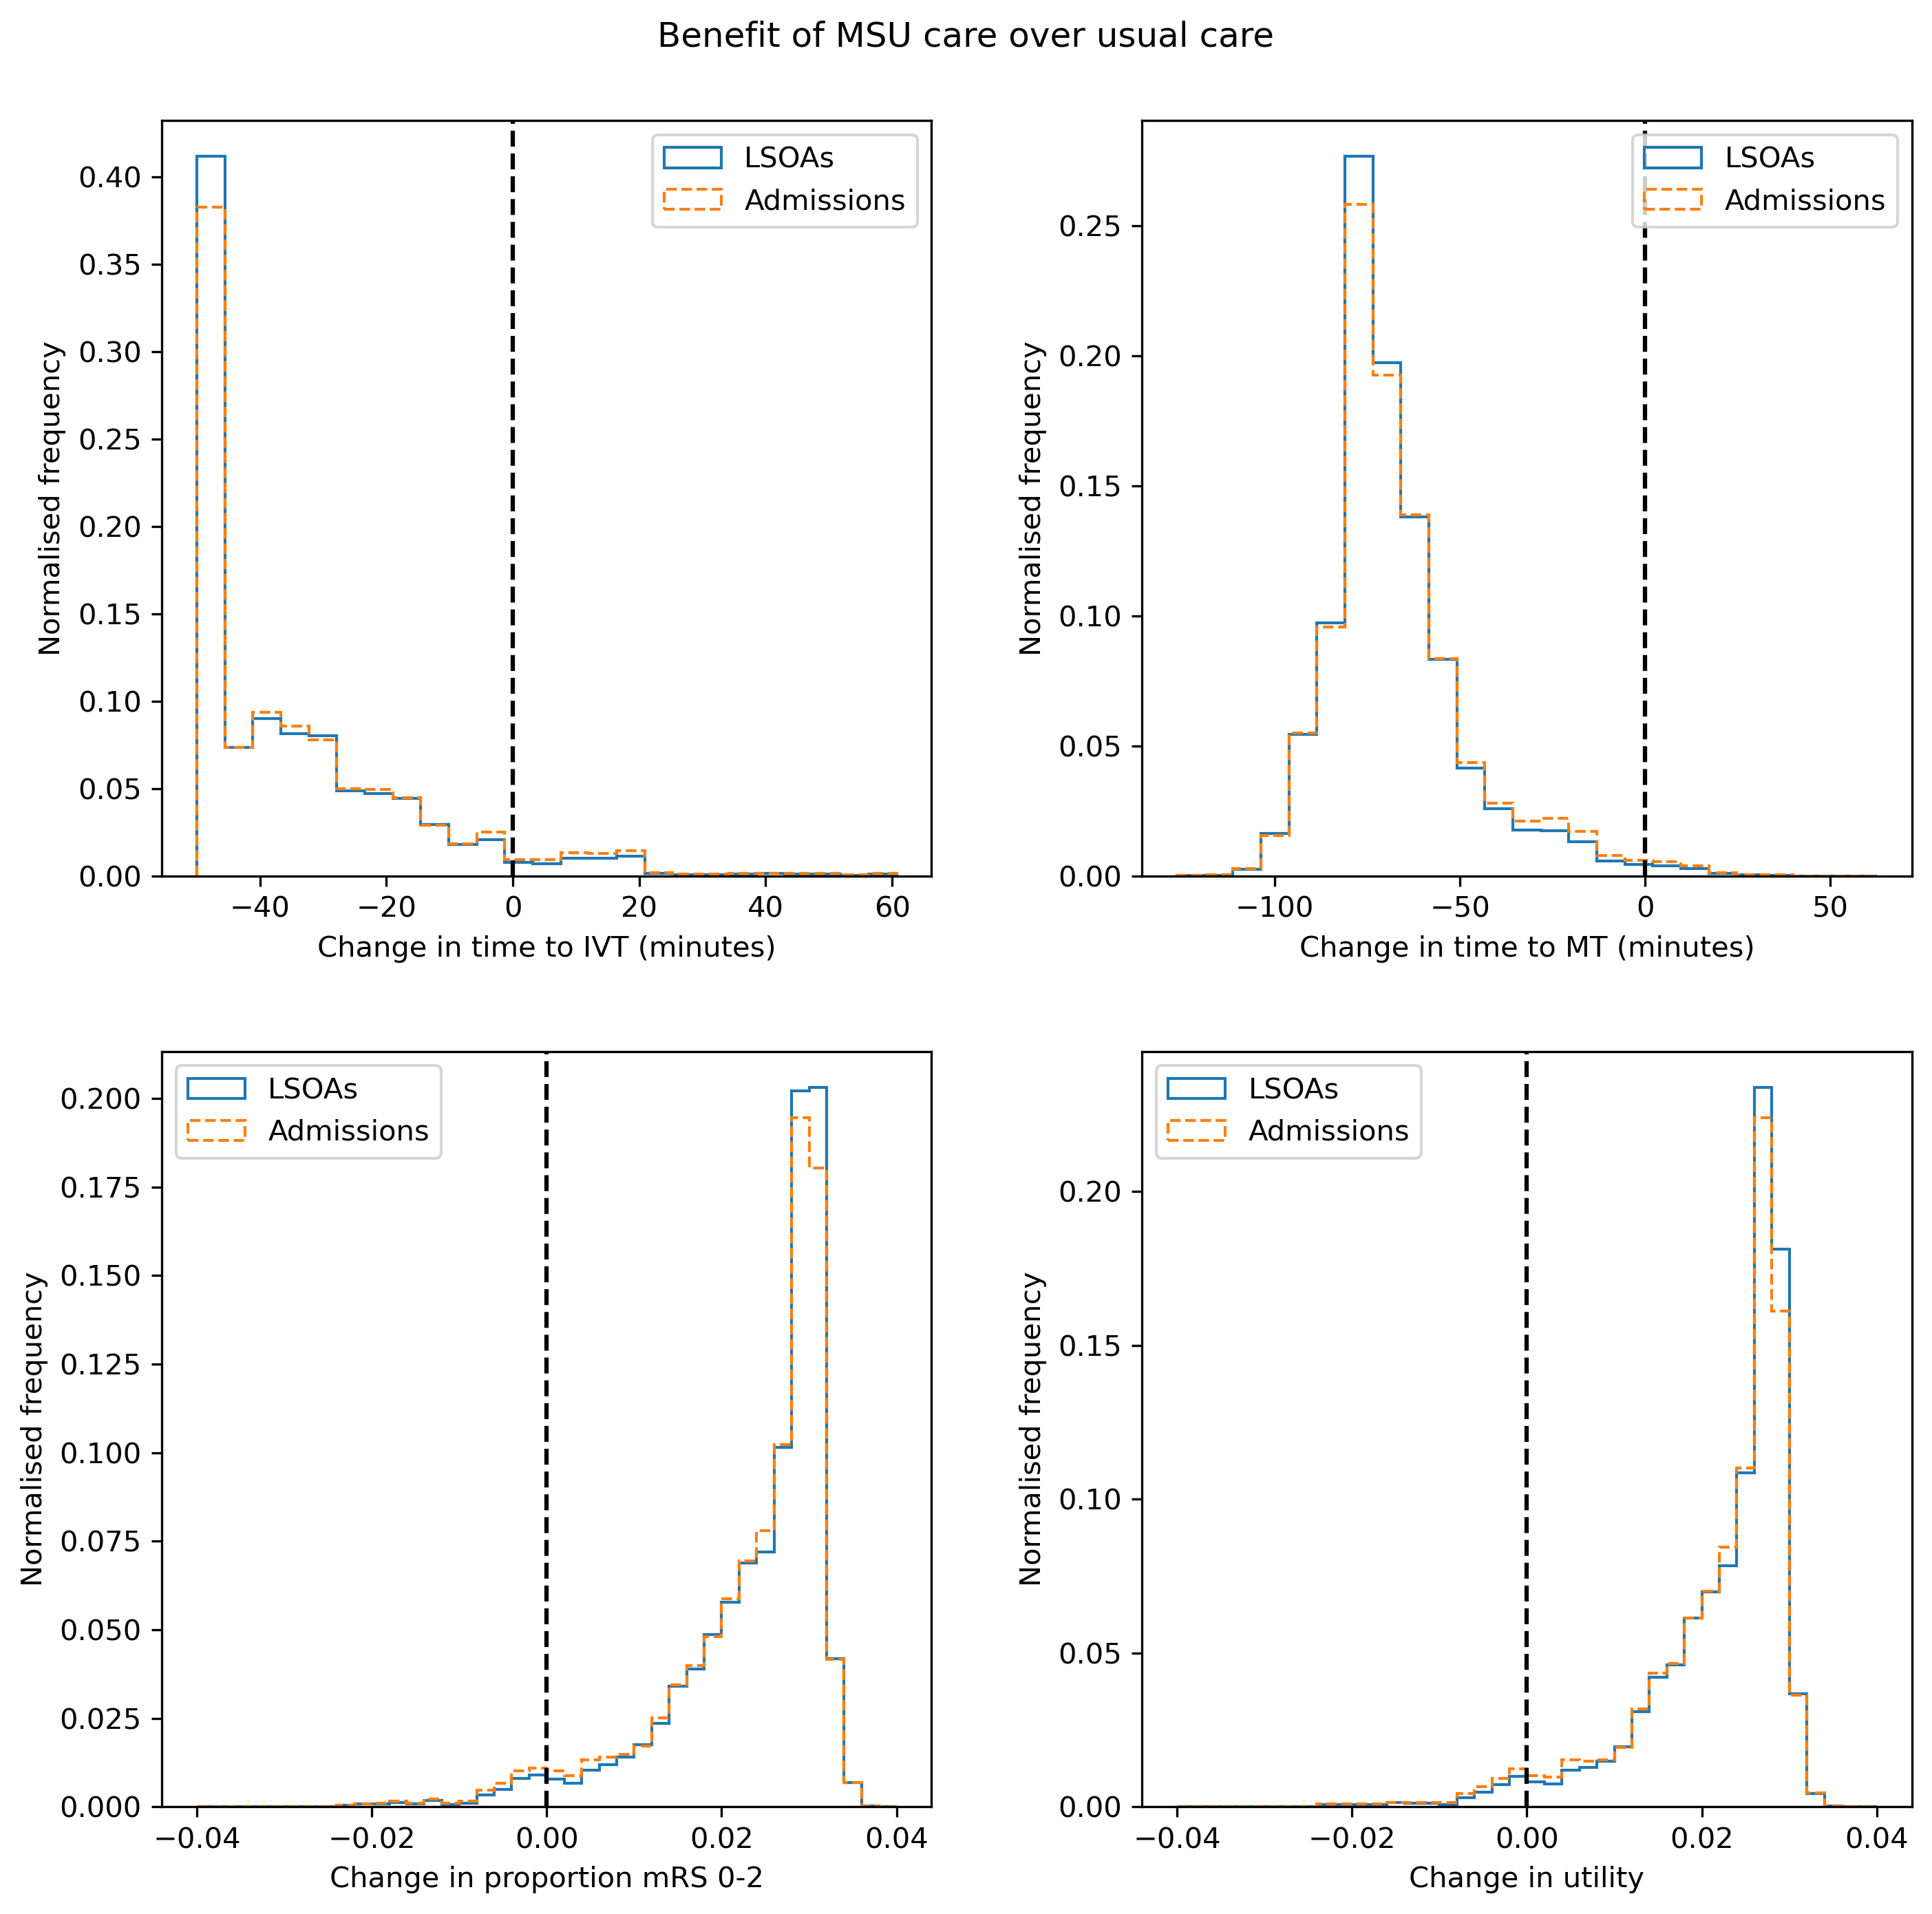
\includegraphics[width=0.75\linewidth]{images/histograms.png}
    \caption{Distribution of benefit of MSU care over usual care across LSOAs (assuming 70\% nLVO, 30\% LVO in the treated population, with LVO receiving IVT/MT in combination). Benefit is described either as even across LSOAs (solid line), or weighted by admissions by LSOA (dotted line). Histograms show change in time to IVT (top left), time to MT (top right), proportion mRS 0-2 post stroke (bottom left), or utility (bottom right).}
    \label{fig:msu_histograms}
\end{figure}

\begin{figure}[h]
    \centering
    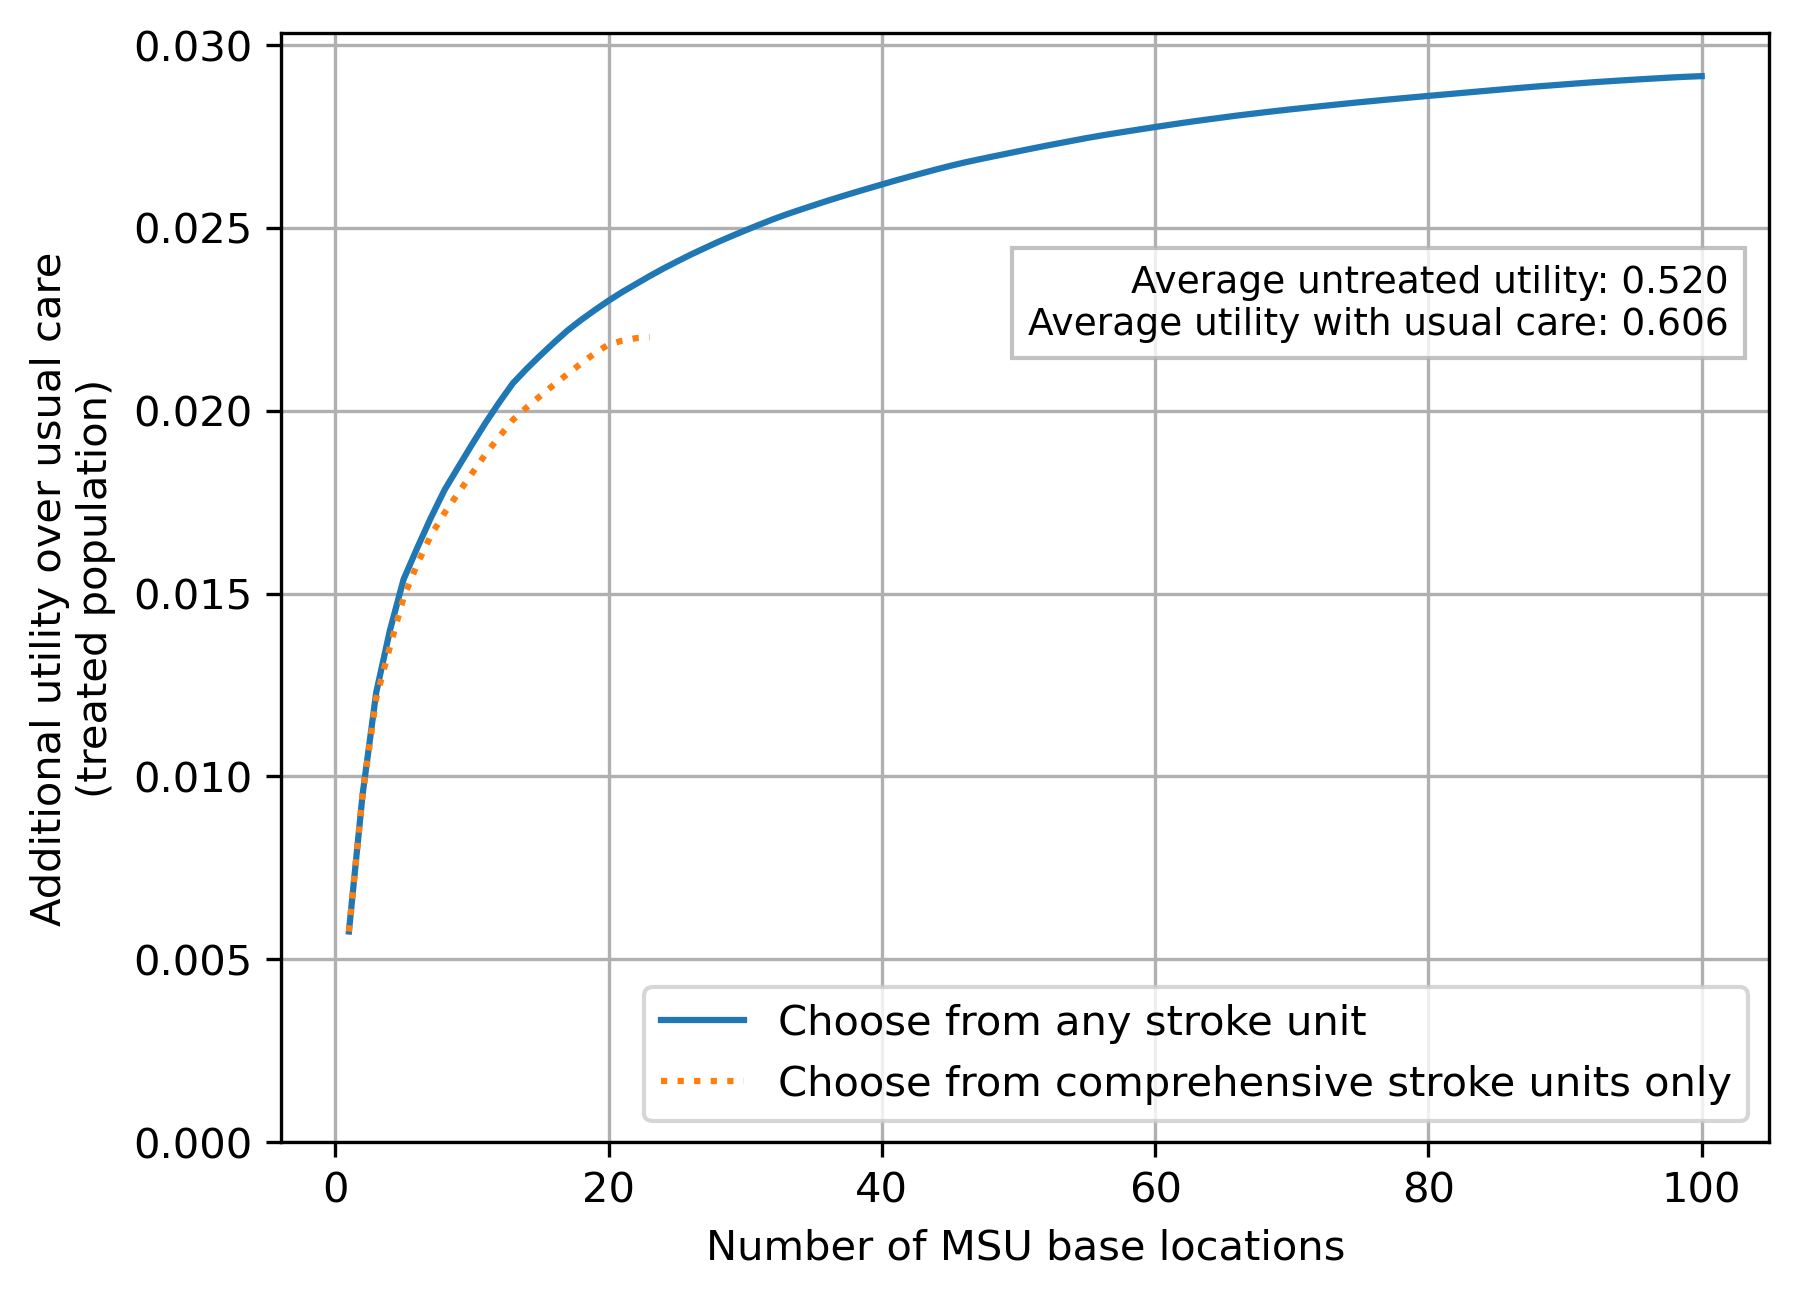
\includegraphics[width=0.5\linewidth]{images/msu_advantages_greedy.png}
    \caption{Increasing number of MSU base locations, with selection by a greedy algorithm based on improvements in utility. The additional utility is for those patients treated by MSU rather than usual care. Units were chosen either from any stroke centre type (solid line) or only from CSCs (dashed line). Utility for the untreated population was 0.520, which was increased to 0.602 with usual care.}
    \label{fig:greedy}
\end{figure}